\begin{center}
    \textbf{\Large Análisis del impacto de la tecnología en la tasa de desempleo:\\Colombia 2000-2020}
\end{center}
%linea horizontal
\begin{center}
	\rule{1\textwidth}{0.5pt}
\end{center}
\vspace{1.5cm}


\textbf{\large 1. Introducción}\\

El desempleo, a pesar de su disminución a través de los años, es un fenómeno que ha afectado a la sociedad Colombiana desde el año 2015 (Vallejo - 2020). En este trabajo se analizará el impacto de la tecnología en la tasa de desempleo en Colombia, para lo cual se utilizará la metodología de la regresión de mínimos cuadrados ordinarios (MCO), la cual permite estimar la relación entre las variables independientes y la variable dependiente, en este caso la tasa de desempleo.\\

EL Banco Mundial define el desempleo como $"$la proporción de la población activa que no tiene trabajo, pero que está dispuesta a trabajar y que está buscando trabajo.$"$ A su vez, las TIC's mediante la innovación y la globalización, están cambiando las forma de trabajo. Por lo que, nos planteamos la siguiente pregunta:

\begin{center}
    ¿Cual fue el impacto de la tecnología dentro de la tasa de desempleo en Colombia?
\end{center}

Existen varios debates con respecto al influjo de las TIC's en el desempleo. Pero nos centraremos en dos: Minian y Monroy (2018) mencionan que el cambio tecnológico realza la productividad y la competencia y desplazan al esfuerzo humano en actividades que las máquinas son más eficientes. Sumado al trabajo de la Organización mundial del trabajo (OIT), donde menciona que a las TIC's como principal causante del aumento de desempleo en el mundo.\\\\


\textbf{\large 2. Revisión de la literatura}\\

Según la Cimoli y Porcile (2013) el desarrollo tecnológico genera efectos positivos en el sector económico, pero existen la disyuntiva entre el efecto que genera este proceso tecnológico dentro del índice desempleo. En este sentido, Minian y Martinez (2018) en su investigación resaltan que, el cambio tecnológico aumenta la productividad y la competitividad, redefine los modelos de producción y desplaza al trabajo humano en actividades que las máquinas pueden hacer de manera más eficiente. Por su lado Alderete (2019), descubre que cuanto más tecnológica es la ciudad mayor es la tasa de desempleo, por lo que existe una correlación negativa entre la tasa de desempleo y la tecnología. \\

Pero se diferencia de la investigación presentada por Orji (2016) donde sustenta que los resultados muestran una relación positiva pero insignificante entre las TIC y la tasa de desempleo.  En esta investigación, el coeficiente de las TIC implica que a medida que el uso de las TIC aumenta en el $1\%$ la tasa de desempleo también aumenta en un $0,09\%$.\\

 Por otra parte, distintos autores consideran que el desempleo obedece a otros criterios económicos mas que al nivel tecnológico, determinando que el desempleo y el empleo con relación a la tecnología dependen del horizonte temporal, así mismo, para este estudio los cambios en el nivel de desempleo no dependen de las inversiones que se hagan en I+D ni mucho menos en la participación creciente del cambio tecnológico. (García, 2013). 

con los expuestos por Aguilera y Ramos (2016) los cuales muestran que los países con altos niveles de PIB per cápita en la región aun se encuentran en una etapa de desarrollo en la que las inversiones en Gasto Interno en ciencia y Tecnología afectan positivamente al empleo, logrando ganancias de productividad, así mismo dado los resultados, se puede afirmar que promover el desarrollo de las innovaciones podría generar impactos significativos en la creación de empleo, lo cual reduce la tasa de desempleo.

¿Afectan las innovaciones tecnológicas al desempleo?, es una de los cuestionamientos que se
realizan muchos autores y que, Matuzeviciute y Buktus (2017) a través de las estimaciones,
excepto una, no sugieren que las innovaciones tecnológicas (aproximadas por familias de patentes triádicas (tfp) tiene un efecto sobre el desempleo. La tercera estimación muestra una correlación negativa, es decir, una mayor actividad de innovación se asocia con una menor tasa
de desempleo. Casi todas las variables de control incluidas en el modelo son estadísticamente
significativas: IED entrante negativamente y IED saliente asociada positivamente con la tasa
de desempleo, el crecimiento económico y un índice de precios más alto, como consecuencia
del crecimiento económico, se correlacionan negativamente con la tasa de desempleo, un gasto
público más generoso sobre el desempleo parece tener un resultado negativo: aumenta el desempleo debido a la reducción de los costos alternativos del trabajo.

Patiño (2014) y Saez (2012) llegan a la conclusión de que existe una relación negativa entre el
progreso tecnológico y el desempleo solo se podría explicar por el dominio del efecto de capitalización, donde menores tasas de crecimiento de la PTF habrían desmotivado la creación de
puestos de trabajo y generado un aumento en el desempleo. Sin embargo, se encontró que, aun
en el caso extremo en que todo el progreso tecnológico hubiera operado bajo este efecto, la desaceleración de la PTF observada durante el periodo 1996-2000 no logra explicar los incrementos en el desempleo, lo que indica que son otros factores, diferentes al progreso tecnológico, los
que explican este fenómeno.

Finalmente, Saka y Othan (2019) en base a los
resultados se obtiene un coeficiente positivo del gasto en I+D que oscila entre 0.012 y 0.034, lo
que significa que la tecnología aumenta el desempleo general. Estos hallazgos también conducen a la importante inferencia de que, en las economías desarrolladas, el progreso tecnológico
hace que la creación de empleo se vea superada por la destrucción de empleo y el mecanismo de
compensación no es eficaz. En general se puede deducir de estudio que, a medida que aumentan
los gastos en I + D, aumenta el empleo de los trabajadores altamente calificados, mientras que
lo contrario es cierto para los trabajadores poco calificados en las economías avanzadas.
\\\\

\textbf{\large 3. Aplicación empírica}\\

\textbf{3.1. Datos}\\

Los datos que se usaran fueron extraídos del Banco Mundial en los periodos anuales 2000 al 2020.

\begin{itemize}
    \item Variable dependiente:
	\begin{center}
	    \begin{tabular}{rcl}
		Y&=& desempleo total ($\%$ de la población activa total).\\ 
	    \end{tabular}
	\end{center}

    \item Variables independientes:
	\begin{center}
	    \begin{tabular}{ccl}
		TIC &=& Importaciones de bienes de tecnologías de la información y\\
			      &&la comunicación (TIC) ($\%$ del total de importaciones de bienes).\\\\
		I &=& Inversión extranjera directa, entrada neta de capital ($\%$ del PIB).\\\\
		IN &=& Logaritmo de la industria, valor agregado ($ \$ $ a precios actuales).\\\\
		FBC &=& Logaritmo de la formación bruta de capital ($ \$ $ a precios actuales).
	    \end{tabular}
	\end{center}
\end{itemize}
\vspace{.5cm}


\textbf{3.2. Metodología}\\

Realizaremos un análisis univariante de la variable dependiente, desempleo total, para definir un modeo ARIMA adecuado mediante su respectivo correlograma y la expresión final del modelo seleccionado.\\

Luego, se modelizará de manera multivariante por MCO la relación entre las variables independientes y la variable dependiente, para determinar la relación entre ellas.\\

Por último, veremos si existe una relación de cointegración entre las variables y en caso de ser así, llevaremos acabo la estimación del modelo de largo plazo.


\begin{table}[!htbp] \centering 
  \caption{Estadísticos descriptivos básicos} 
  \label{} 
\begin{tabular}{@{\extracolsep{5pt}}lcccccc} 
\\[-1.8ex]\hline 
\hline \\[-1.8ex] 
Statistic & \multicolumn{1}{c}{N} & \multicolumn{1}{c}{Mean} & \multicolumn{1}{c}{St. Dev.} & \multicolumn{1}{c}{Min} & \multicolumn{1}{c}{Median} & \multicolumn{1}{c}{Max} \\ 
\hline \\[-1.8ex] 
Y & 21 & 11.371 & 2.961 & 8.300 & 10.490 & 20.520 \\ 
TIC & 21 & 10.006 & 1.071 & 8.500 & 9.902 & 13.037 \\ 
I & 21 & 3.709 & 1.196 & 1.818 & 4.055 & 7.029 \\ 
lnIN & 21 & 24.874 & 0.531 & 24.009 & 25.078 & 25.553 \\ 
lnFBC & 21 & 24.539 & 0.610 & 23.423 & 24.774 & 25.239 \\ 
\hline \\[-1.8ex] 
\end{tabular} 
\end{table}

Notemos que en todas las variables a estudiar, la media y la mediana tienen datos próximos entre si, por lo que los datos no son atípicos.

\begin{table}[!htbp] \centering 
  \caption{Gráficos temporales} 
  \label{} 
\begin{multicols}{2}
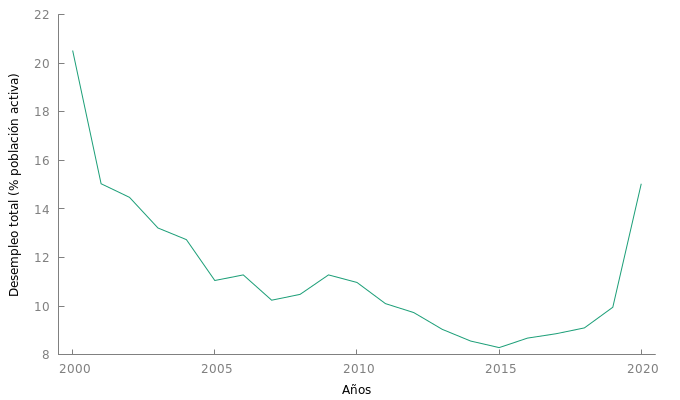
\includegraphics[scale=.33]{r/econometria2/image/desempleo.png}\\
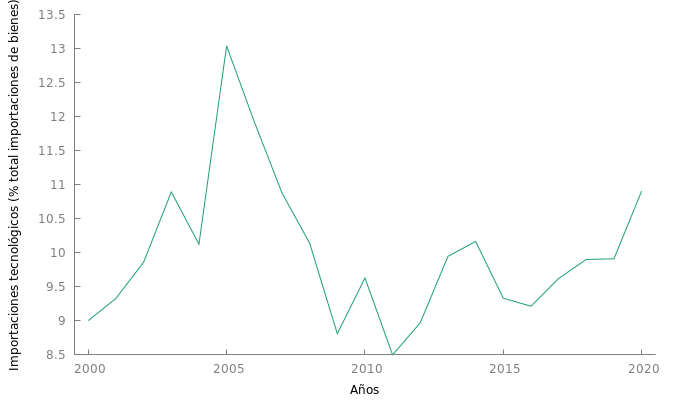
\includegraphics[scale=.33]{r/econometria2/image/TIC.png}\\
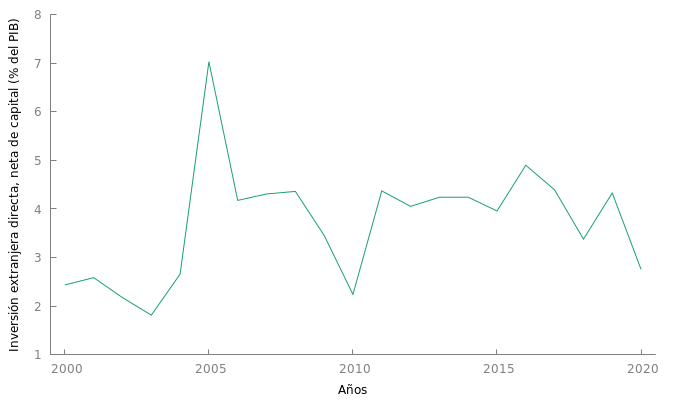
\includegraphics[scale=.33]{r/econometria2/image/I.png}\\
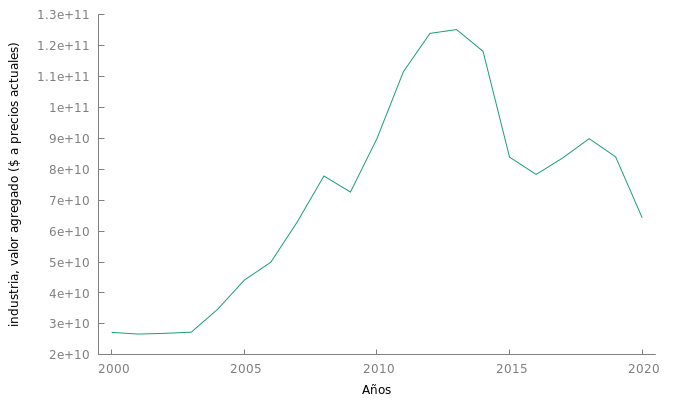
\includegraphics[scale=.33]{r/econometria2/image/IN.png}\\
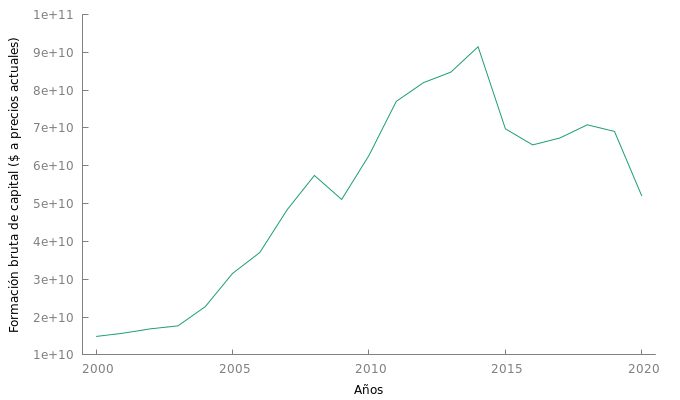
\includegraphics[scale=.33]{r/econometria2/image/fbc.png}\\
\end{multicols}
\end{table}


\textbf{3.2.1. Univariante}\\

Realizamos primero el test de Dickey Fuller donde aceptamos la hipótesis nula de que la serie es no estacionaria, por lo que se procede a realizar la transformación a logaritmos, de donde ya podemos rechazar la hipótesis nula a un $5\%$. Luego elegimos un modelo ARIMA(1,2,1), donde 

\textbf{3.2.2. Multivariante}\\

Modelización MCO de la relación entre las variables. 

\textbf{4. Conclusiones}\\

\textbf{5. Bibliografía}\\
\begin{itemize}
    \item Álvarez, N., y Aldarete, M. V. (2019). Ciudades innovadoras: el efecto sobre el desempleo en la región de Latinoamérica. Trilogía Ciencia Tecnología Sociedad, 193-222.
    \item Banco Mundial. (2013, Septiembre 10). Conectarse para trabajar: Cómo las TIC amplían las oportunidades de empleo en todo el mundo.
    \item Cueva, J. Vivanco, F. Yunga, C. Tapia. Impact of Technology on the unemployment rate: Analysis for Latin American countries in the period 2000 – 2018. \url{http://dx.doi.org/10.54753/suracademia.v9i18.1399}
    \item L. E. Vallejo Zamudio. Repercusiones del desempleo en la estructura productiva colombiana \url{https://doi.org/10.19053/01203053.v39.n70.2020.12035}
    \item M. Cimili y G. Porcile. Tecnología, heterogeneidad y crecimiento: una caja de herramientas estructuralistas. \url{http://hdl.handle.net/11362/4592}
    \item Minian, I., y Martinez, A. (2018). El impacto de las nuevas tecnologías en el empleo de México. Revista Problemas del desarrollo, 1-20.  \url{http://dx.doi.org/10.22201/iiec.20078951e.2018.195.64001}
    \item Techcetera. (2012, Noviembre 27). La tecnología como causante del desempleo: un enorme reto para la humanidad. Retrieved from Techcetera: \url{https://techcetera.co/la-tecnologia-como-causante-de-desempleo-un-enorme-reto-para-la-humanidad/}
\end{itemize}


\textbf{6. Anexos}\\

\begin{center}
Modelo: ARIMA, usando las observaciones 2002--2020 ($T$ = 19)\\
Variable dependiente: $(1-L)^2$Y\\
Desviaciones típicas basadas en el Hessiano

\vspace{1em}

\begin{tabular}{lr@{.}lr@{.}lr@{.}lr@{.}l}
  &
 \multicolumn{2}{c}{Coeficiente} &
  \multicolumn{2}{c}{Desv.\ Típica} &
   \multicolumn{2}{c}{$z$} &
    \multicolumn{2}{c}{valor p} \\[1ex]
const &
  0&487815 &
    0&295962 &
      1&648 &
        0&0993 \\
$\phi_{1}$ &
  $-$0&947063 &
    0&111223 &
      $-$8&515 &
        0&0000 \\
$\theta_{1}$ &
  0&711938 &
    0&338656 &
      2&102 &
        0&0355 \\
\end{tabular}

\vspace{1ex}
\begin{tabular}{lrlr}
Media de la vble. dep. &  0.555789 & D.T. de la vble. dep. &  1.646937 \\
Media de innovaciones &  0.037723 & D.T. innovaciones &  1.437607 \\
$R^2$ &  0.443565 & $R^2$ corregido &  0.410834 \\
Log-verosimilitud & $-$34.22447 & Criterio de Akaike &  76.44895 \\
Criterio de Schwarz &  80.22670 & Hannan--Quinn &  77.08829 \\
\end{tabular}


\vspace{1em}

\begin{tabular}{llrrrrr}
& & & Real & Imaginaria & Módulo & Frecuencia \\ \hline
AR \\ 
& Raíz & 1 & $-1.0559$ & $0.0000$ & $1.0559$ & $0.5000$ \\ 
MA \\ 
& Raíz & 1 & $-1.4046$ & $0.0000$ & $1.4046$ & $0.5000$ \\ \hline
\end{tabular}

\end{center}
